% ------ METADATA ------
\newcommand{\bookauthor}{Эмиль~Весна}
\newcommand{\booktitle}{ГУЦИНЬ С~МИЛЛИОНОМ~СТРУН}
\newcommand{\bookstarted}{неизвестно}
\newcommand{\bookfinished}{пока нет}
% ------ METADATA ------

% ----- XELATEX SYMBOL -----
\usepackage{xltxtra}
% ----- XELATEX SYMBOL -----

% ----- HYPHENATION -----
\usepackage{hyphenat}
% ----- HYPHENATION -----

% ----- GEOMETRY -----
\usepackage[left=1.5cm,right=1.5cm,top=2cm,bottom=2cm,bindingoffset=0.5cm]{geometry}
% ----- GEOMETRY -----

% ----- INCLUDE PDF AS PAGES -----
\usepackage{pdfpages}
% ----- INCLUDE PDF AS PAGES -----

% ----- DROPPING CAP -----
\usepackage{type1cm,lettrine}
% ----- DROPPING CAP -----

% ----- FONTS -----
\renewcommand{\baselinestretch}{1.2}
\setmainfont{Linux Libertine}
% ----- FONTS -----

% ------ HYPERLINKS ------
\usepackage{hyperref}
\definecolor{LinkColor}{HTML}{0969DA}
\hypersetup{colorlinks=true, linkcolor=LinkColor, citecolor=LinkColor, filecolor=LinkColor, urlcolor=LinkColor}
% ------ HYPERLINKS ------

% ------ FANCY PAGE STYLE ------
\setlength{\headheight}{15pt}
\usepackage{fancyhdr}
\pagestyle{fancy}
\fancyhead[LE,RO]{\thepage}
\fancyhead[LO]{{\small\textsc{\booktitle}}}
\fancyhead[RE]{{\small\textsc{\bookauthor}}}
\fancyfoot{}
    \fancypagestyle{plain}{
    \renewcommand{\headrulewidth}{0mm}
    \fancyhead{}
    \fancyfoot{}
}
% ------ FANCY PAGE STYLE ------

% ------ ELEMENTS ------
\newcommand{\asterism}{\vspace{1em}{\centering\Large\bfseries$\ast~\ast~\ast$\par}\vspace{1em}}
\newcommand{\FM}{\footnotemark}
\newcommand{\FA}[1]{\footnotetext{#1 \emph{\ml{$0$}{---~Прим.~авт.}{---~Author.}}}}
% ------ ELEMENTS ------

\begin{document}

% ----- FRONT COVER -----
% \includepdf[pages={1}]{\coverfrontfilename}
% ----- FRONT COVER -----

% ----- EMPTY PAGE -----
% \newpage\thispagestyle{plain}~
% ----- EMPTY PAGE -----

% ------ TITLE PAGE ------
\begin{titlepage}
{
\centering
{~\par}
\vspace{0.25\textheight}
{\LARGE\bookauthor\par}
\vspace{1.3cm}
{\Huge\textbf{\booktitle}\par}
\vfill
{\includegraphics[width=6em]{\publisherlogofilename}\par}
}
\end{titlepage}
% ------ TITLE PAGE ------

% ----- TRIGGER WARNING -----
% \newpage\thispagestyle{plain}
% {~\par}
% \vfill
% {\centering
\includegraphics[width=4em]{tw.pdf}\par}
% \vspace{1em}
% {\centering\Large\strong{\ml{$0$}{Предупреждение}{Content Warning}}\par}
% \vspace{0.5em}
% {\centering\large{Данное произведение содержит описание неизлечимых болезней, психических состояний, врачебных манипуляций, упоминания суицида, химических зависимостей, сцены насилия и убийств, мат, а также гомофобную, трансфобную, сексистскую и расистскую лексику.}\par}
% \vfill
% {~\par}
% ----- TRIGGER WARNING -----

% ----- TABLE OF CONTENTS -----
\tableofcontents
% ----- TABLE OF CONTENTS -----

\pagestyle{fancy}


\section{<<Когда-нибудь тёмною ночью...>>}

\begin{verse}
Когда-нибудь тёмною ночью\\
Заплачу над кровью пролитой,\\
Когда не останется мочи,\\
Когда опустеют молитвы,

Когда все надежды издохнут,\\
Когда я дойду до границы,\\
Найди меня, нежная кроха,\\
И мне помоги не свалиться.

\emph{Октябрь 2012}
\end{verse}
\newpage

\section{П. К.}

\begin{verse}
С зелёной книжкой и вопросом\\
Глаза раскосые у двери.\\
Я, возомнив себя колоссом,\\
На помощь бросился, не веря.

Тиха всё так же зелень сада,\\
Снега всё так же белоснежны,\\
А очи лисьи всюду рядом ---\\
Молчат и зрят спокойно-нежно.

\emph{2012}
\end{verse}
\newpage

\section{Песня о Хелависе}

\begin{verse}
Зазвенели тихо струны:\\
С маком алым у чела\\
Сероглазая колдунья\\
Песню арфою ткала.\\
Огонёк свечи усталой\\
Жёг полночную вуаль.\\
К звёздам песня улетала,\\
Пыльный шлях стремился вдаль.

А вдали, не зная страха,\\
Тьму кирасой распоров,\\
Рыцарь шёл с войны по шляху,\\
Вёл лошадку без подков.\\
Он во Франции далёкой\\
Воевал за короля.\\
Нажил серебра немного,\\
Шрам приметный от копья.

Песня нежно-величаво\\
Душу тронет, как струну.\\
Вдруг крылом взовьётся арфа,\\
Волком взвоет на луну\\
И замолкнет...\\
Стук, как в сердце,\\
Мягкий и усталый взгляд:\\
<<Дай, хозяюшка, согреться...\\
Спой, голубушка, на лад...>>

С тихой ночи новолунья\\
Год прошёл, второй бежит.\\
Сероглазая колдунья\\
Колыбельку сторожит.\\
Пламя свечки пляшет зыбко,\\
Песня та же на устах,\\
Рыцарь слушает с улыбкой,\\
И молчит угрюмо шлях...

\emph{1 марта 2012}
\end{verse}
\newpage

\section{Лунные сады}

\begin{verse}
В холодном небе, на лунных склонах,\\
Над зеркалами семи морей\\
Есть сад укромный, где яблонь кроны\\
Земных прекрасней, земных пышней.

Там ночь тиха, и шагов не слышно,\\
Но лишь эол посетит тот сад ---\\
Малинник пышный и листья вишни\\
Сусальным золотом зазвенят.

И век за веком идёт неспешно,\\
Осенний день переходит в вешний.\\
А сад и осенью, и зимой\\
Звенит своей листвой.

Там девы рыщут, и нет их краше,\\
Шуршит их платьев паучий шёлк.\\
Хоть нет там стражи, но, воля ваша,\\
Их плен снести даже я б не смог.

Ведь нет на землю пути-дороги,\\
Сердца красавиц тоской полны.\\
Бегут эпохи, летят эпохи,\\
А девы бродят в саду Луны...

И век за веком идёт неспешно,\\
Осенний день переходит в вешний.\\
А девы плачут, а девы ждут,\\
Что их спасти придут.

\emph{4 декабря 2012}
\end{verse}
\newpage

\section{Есенинские мотивы}

\begin{verse}
Закурился дымок за околицей,\\
Сладок свет одурманенных звёзд.\\
Колоса, как пустынники, молятся\\
Тихим шелестом бронзовых кос.

Ты, Россия моя, исстрадалася,\\
Задыхаясь под гнётом плетей.\\
Чтоб работалось мне, чтоб мечталося,\\
Покурить выхожу за плетень.

Как дымок, уплывают мгновения,\\
И напишет историю тлен,\\
Как пропащее то поколение\\
Поднимало Россию с колен.

\emph{29 марта 2013}
\end{verse}
\newpage

\section{Марина}

\begin{verse}
Цветами увита лесными,\\
Танцуешь во мраке ночном.\\
Твоё белопенное имя\\
Играет луны серебром.

Представлю, что где-то ты рядом ---\\
И сердце уходит в полёт...

Как жаль, что ни словом,\\
ни взглядом\\
Судьба нас с тобой не сведёт.

\emph{2013}
\end{verse}
\newpage

\section{Быть может (M. R.)}

\begin{verse}
Однажды в вечер, ненастный ветер,\\
Горячего жаждущий чаю,\\
Немытый, небритый,\\
Дорогой разбитый,\\
Быть может, тебя повстречаю.

Ты скажешь, может, что так негоже ---\\
Консорту бродить по трущобам.\\
Отвечу: не принцем\\
Посмел я явиться,\\
А старым, больным и недобрым.

Ты скажешь: поздно, завяли розы,\\
Но ты заходи, весь иссох ведь.\\
Готовлю я редко,\\
Сижу на таблетках,\\
Чтоб ночью с тоски не издохнуть.

И дождь зашепчет шуршащей речью,\\
И чайничек свистнет упруго...\\
А мы терпеливо под ветра порывы\\
Излечивать будем друг друга.

\emph{2013}
\end{verse}
\newpage

\section{Голос}

\begin{verse}
В тёмной ночи и светлым днём,\\
Среди леса и стен бетонных\\
Древний голос гремит как гром,\\
Через сон пробиваясь стоном.

Заставляет мечтать об одном,\\
Добавляя к нему <<всего лишь>>.\\
Не запьёшь этот голос вином,\\
Не закуришь и не заколешь.

Он всегда, отличив средь лжи\\
Настоящее, неподдельное,\\
Прекращает греметь, лежит\\
И мурлычет в моей постели.

\emph{22 сентября 2013}
\end{verse}
\newpage

\section{Осень (акростих)}

\begin{verse}
Слетел последний лист осенний,\\
А осень, хладна и гола,\\
Шатаясь в дымке серой лени,\\
Амриту мне преподнесла.

Я ж, пригубив её от края,\\
Ночами крепче начал спать,\\
Как пчёлка, досыта вкушая\\
Объятий сладостную падь.

Водой ноябрь утекает,\\
Свистит эол во весь карниз...\\
Кудахчут: <<Осень не такая>>,\\
А я курю у двери рая,\\
Я счастлив. Впереди --- лишь высь.

\emph{Ноябрь 2013}
\end{verse}
\newpage

\section{Sunrise}

\begin{verse}

% х7700х = А1
% хх0770 = А2
% 3200хх = А3
% 2200хх = А4
% хх2102 = А5
% хх2100 = А6
% хх4304 = А7
% хх4302 = А8
% 8700хх = А9

% А1
Purple sunrise\\
% А2
Promise of night\\
% А1 	А2
That might be true at the morning\\
% А3 	А4
Wise of the wind\\
% А1
I heard from you\\
% А3 	А4 	А1
In the whisper of silently sorrow

% Bridge #1:
% х7х007
% х5х005
% х3х003
% х2х003 (2 раза)
% А3 А4 А1 (2 раза)

Fondness of silk\\
Hides in your lips\\
That were like stone at the evening\\
It was your words\\
Your only words\\
You said ``My darling, don't leave me''

% Bridge #2:
% ххх00(12)
% ххх00(14)
% ххх00(15)
% ххх00(14) (2 раза)
%
% Bridge #1.
%
% А5 А6 А7 А8

% А5 	А6
Purple sunrise\\
% А7 	А8
Destiny's dice\\
% А5 	А6 	А7 	А8
Who threw them down so careless?\\
% А3 	А4
Time is so slow\\
% А1 	А9
I fell in love\\
% А3 	А4 	А1 	А9
And forgot all my success and failures.

% хх4230
% хх0230
% 3200хх
% А9
% хх4230
% хх0230
% 3200хх
% х3201х
%
% Бой на верхних струнах восьмыми:
% G A4 Em C
%
% Финальный – G снизу вверх.
\emph{2014?}
\end{verse}
\newpage

\section{Hrorek}

\begin{verse}
% Em 	Am 	Em 	C
Water's been cutting by dragonboat\\
% D 	Hm 	Em
Sky is so close to bow\\
What are you thinking about, my \textit{konung}?\\
Sun rose an hour ago\\
% G 	D
Wind's favorable for Hrorek\\
% Am 	Em
And Master of Water is kindly too\\
% C 	D 	G
Oars like seagulls are stroking the waters\\
% D 	Hm 	Em
And nothing but silence reigns over the crew

% Chorus:
% G 	Hm 	F#m
Could you ever know that your greedy son (torn apart with trees)\\
% E 	G
He shall give birth to the greatest conqueror\\
% D 	A
Who's name's full of glory and sanctity?\\
% G 	Hm 	F#m
Could you ever know that your clan will rule \textit{Ostland} (eight hundred years)\\
% E 	G
All you could know is you dare\\
% D
And that is it

Banished away by your own brother\\
How could you rise and survive?\\
There's in your hands the Slavian charta\\
Suggestion to govern their lifes\\
Wind's favorable for Hrorek\\
\textit{V\'{o}lkhov} is front, and \textit{Nev\'{a}} is behind\\
Dragon went out to the calm water\\
% Hm 	F#m 	E
Shadows of future don't trouble your mind\\
anymore

% Chorus:
Could you ever know that your great-grandson (born in the storm)\\
Built his great power on bones of men\\
He will be gone playing game of chess?\\
Could you ever know that your clan will live in \textit{Ostland} (like in your home)\\
All you could know is you can\\
And that is it

\emph{2014?}
\end{verse}
\newpage

\section{Последний бой}

\begin{verse}
% Am 	D 	Am
Мой меч --- искра пылающей мести,\\
Мой путь --- лишь нить полотна дорог.\\
Мой шаг --- печаль и дурные вести,\\
Мой дух покинул этот мирок.

% G 	D 	Em
Мы идём на последнюю битву,\\
Мы поём --- враг читает молитвы.

Мой дом --- два камня и пепелище,\\
Мой пёс лежит, разинувши пасть.\\
Мой род победы больше не ищет,\\
Мой род пощады больше не даст.

Мы идём на последнюю битву,\\
Мы падём, но не будем забыты.

Мой зов --- не жизни, смертного боя.\\
Мой сын носить не будет оков.\\
Мой тыл жена прикроет собою,\\
Мой род меня прикроет с боков.

Мы идём на последнюю битву,\\
Мы падём, но не будем забыты.\\
Мы идём на последнюю битву,\\
Воспоют нас поэты врагов.

\emph{01.07.2015}
\end{verse}
\newpage

\section{Дракон, дочь дракона}

\begin{verse}
В Междумирье, под светом неведомых звёзд,\\
Где обитель лежит для ещё не рождённых,\\
Дремлют очи, как пламя рубиновых роз\\
До поры свито в камень в закрытых бутонах.

Вечность --- миг, и Вселенная --- точка для вас,\\
Что ещё не познали ни света, ни боли.\\
Но я знаю --- под гнётом драконовой воли\\
Ты родишься. Придёт тот неведомый час ---

Пламя гор заструится горячею кровью,\\
И алмаз трансмутирует в нежную плоть,\\
Чешуя станет кожей, а злоба --- любовью...\\
И никто нас не сможет тогда побороть.

Я открою тебе тайны моря и неба,\\
И на струнах светила играть научу.\\
Силе крыльев твоих, словно гамма-лучу,\\
Будут тонкой бумагой реальность и небыль.

А когда час придёт мне уйти на простор ---\\
Твоё пламя зажжёт погребальный костёр.

\emph{2014}
\end{verse}
\newpage

\section{Сердце Земли}

\begin{verse}
Город утих,\\
Звёзды зажглись,\\
Рокот машин угасает вдали.\\
Лес пригорюнился, тёмен и лыс,\\
Бьётся лишь сердце Земли.

Войны грохочут,\\
Стонет солдат,\\
Почву снаряды как плуги рыхлят.\\
Но,\\
Лишь утихнет последний снаряд,\\
Слышен всё тот же набат.

Старый шаман\\
В бедном типи\\
Дождь вызывает дымом костра.\\
И, лишь ребёнок во сне засопит,\\
Слушает стук до утра.

Слышал ли ты\\
(Может, и нет),\\
Как, сотрясая кромешный гранит,\\
Ровно, легко, далеко в глубине\\
Сердце планеты звенит?

\emph{2014}
\end{verse}
\newpage

\section{Ведьма}

\begin{verse}
Измазал чернилами небо Господь,\\
Рассыпал алмазную звёздную пыль,\\
Разлил молоко... нет, безумец, погодь,\\
То сказка. А я расскажу тебе быль.

Шёл странник из северных сумрачных стран,\\
Котомку с провизией нёс на плече.\\
Порою от старых он морщился ран,\\
Свой мех наполняя в хрустальном ключе.

Шёл утром, и днём, и весь вечер он брёл,\\
И ел на ходу, и на солнце глядел,\\
Всё ждал --- из-за дальних покажется дол\\
Его деревушка, родимый удел.

Но ночь наступила, и месяц златой\\
Повис на чумазом небесном котле.\\
Меж сосен, блестевших резною корой,\\
Лёг спать бедный странник на голой земле.

И снится ему, что седой серафим\\
С заоблачных высей на землю сошёл,\\
Сияя, как солнце, склонился над ним,\\
И шёпот, как колокол, звонок и зол:

<<Пришло твоё время, раб Божий, пришло!\\
Не взяться тебе за твоё ремесло!\\
Ты выжил в войне, пережил десять ран,\\
Но вышел срок жизни, что Богом был дан!>>

Виденье растаяло. Путник лежал,\\
Обдумывал странный, пугающий сон...\\
Вдруг ветер заохал, потом завизжал...\\
И волки завыли вблизи в унисон.

Вмиг вспомнил воитель ночные бои:\\
Со скрежетом вышел из ножен кинжал,\\
Златым фейерверком сверкнули кремни,\\
И факел смолистый огнём запылал!

Подходят всё ближе, всё ярче блестят\\
Клыки белой соли, кровавого камня...

Услышал вдруг воин сквозь воющий ад\\
Знакомую тень своей трепетной лани:

<<Я долго молилась с рыданьем любви,\\
Совсем потерявши надежду и сон.\\
На рынке, у старой гадалки-змеи\\
Случайно узнала, что срок твой сочтён.

Я ведьмою стала, к чертям воззвала,\\
И я не позволю тебе умереть.\\
Мне жизнь без тебя, верный друг, не мила.\\
Будь проклят тот Бог,\\
Что предрёк тебе смерть!>>

И робкое солнце над светом над белым\\
Взошло, освещая запущенный дом.\\
Поляна пуста.\\
Ни следов и ни тела.\\
И лишь пентаграмма пылает огнём.

\emph{2016}
\end{verse}
\newpage

\section{Печальная песня Гурни Халлека}

\begin{verse}
Полногрудые гурии тают\\
Словно мёд под моими руками,\\
Тихий шёпот весеннего сада\\
Разливает сиянье вокруг.\\
Ну а сердце осталось в пустыне,\\
Моё сердце осталось в пустыне,\\
В старом, душном, седом Арракине,\\
Где сложил свою голову друг.

Как лоза виноградная, манят\\
И ласкают прекрасные длани,\\
И скрываются нежности рая\\
В приоткрытых, как роза, устах.\\
Отчего же твержу я о битвах,\\
Отчего же твержу я о битвах,\\
О горах, что песками покрыты,\\
Отчего засыпаю в слезах?

В кубке хмель звонкой рыбкою плещет,\\
Обнажённые нежные плечи,\\
Жемчугами заморскими блещет\\
Золотая плетёная нить...\\
Ну а сердце осталось в пустыне,\\
Моё сердце осталось в пустыне,\\
И не может вино и в помине\\
Мою горечь теперь утолить.

\emph{1 июля 2016}
\end{verse}
\newpage

\section{Странница}

\begin{verse}
 Обними меня, странница-дева,\\
И рубаху накинь мне на плечи.\\
Идентичны и право, и лево,\\
Если вместе. И сложное --- легче.

А рубаха из белого шёлка,\\
И нежнее не видывал прежде.\\
Хоть колючи укоры иголок,\\
Но иголки пестуют одежду.

Не спасает рубаха от ливня,\\
Но похоже ль, что ливня боюсь я?\\
Моей шее железная гривна,\\
Что твоей --- изумрудные бусы.

Обними меня, воин покоя,\\
Наточи свою нежность рукою,\\
Позабудь все стихи и молитвы ---\\
Это я, твоя главная битва.

\emph{17 октября 2017}
\end{verse}
\newpage

\section{Призрак весны (f\"{u}r M. R.)}

\begin{verse}
Морозные утра вдруг канули в Лету.\\
И дождь, и в тумане собор.\\
Хоть мудрый весной я, поверьте --- не в эту.\\
А впрочем, о чём разговор.

Эсминец дрейфует в балтийском тумане.\\
Ликует маяк; не угас\\
Ревущий белугой пылающий пламень.\\
О боже, о чём я сейчас.

Закатные речи на темы, что стары\\
Едва ли как мир или пыль.\\
Немые печали и уголь гитары,\\
Болота и флюгерный шпиль...

Едва ли я помню слова --- это призрак,\\
едва ль искушён я в словах,\\
Рождённых, как память, мечта или вызов,\\
Гореть и сгорать в головах.

\emph{9 марта 2018}
\end{verse}
\newpage

\section{Зимняя вишня}

\begin{verse}

К чему теперь споры?\\
К чему разговоры?\\
Не фениксы люди --- из пепла восстать!\\
Не звери, не люди поганые воры:\\
Россию --- по прутьям, коль нечего брать!

К чему теперь речи и пышные встречи?\\
За нас ли ты топишь, играя мечом?\\
Тяни свои трели!\\
А дети сгорели.\\
Пускай.\\
Нарожают солдатки ещё.

Вы можете плакать с букетами маков,\\
Испортив красивый пост-выборный вид,\\
Не фениксы люди.\\
Их больше не будет.

<<Людей не хватает. Россия горит>>.

\emph{27 марта 2018}
\end{verse}
\newpage
\section{Хватит}

\begin{verse}
Хватит слов, откровенности, лжи.\\
Я достаточно фраз намерил.\\
Мне бы лечь в переспелой ржи\\
(не над пропастью)\\
И поверить.

Хватит связками воздух вить.\\
Лишь прикрытием служит слово.\\
Я забыл, что такое любить.\\
Я забыл, как хотеть другого.

Хватит звуков. Уже не юн\\
Соловей, что слетел с насеста.\\
Я --- гуцинь с миллионом струн.\\
Я пою под руками маэстро.

И не надо, прошу, не плачь\\
И не жалобь тоскливым взглядом!\\
Хоть для многих я --- недоврач,\\
Я был доктором больше, чем надо.

Хватит слов, обещаний, слёз.\\
Я --- молчанье.\\
Я --- голос Бога.\\
Если сможешь --- коснись волос.\\
Или топай своей дорогой.

\emph{30 мая 2018}
\end{verse}
\newpage

\section{Отголосок зимы}

\begin{verse}
Мне трудно петь.\\
Слова застревают в горле.\\
И утро не в радость, и вечер уже не в счёт.\\
Гитара фальшивит,\\
Лады все струнами стёрло,\\
И кровь рекою вспять куда-то течёт.

И в сны прокралась\\
Несчастная та глупышка,\\
Что в снах обнимает и ненавидит днём.\\
Утром я в страсти,\\
А вечером --- в книжках.\\
Имя забывши, мечтаю перед окном.

А лето цветёт,\\
Луна меняет фазы,\\
Как дева --- браслеты: на каждые сутки --- свой.\\
Наша любовь ---\\
Это комедия, маразм.\\
Но на смех не тянет, кроме ухмылки кривой.

Я тебя позабуду.\\
Я обещаю, сокол.\\
Ты мне не будешь сниться, я тушей не буду гнить.\\
Я лишь надеюсь:\\
Несчастной моей любовью\\
Я сделал прочнее твою непрочную нить.

Я грусть не сниму,\\
Я в ней попытаюсь греться.\\
Я завернусь, как в шарф, в твой остывший след.\\
Но, видно, тому,\\
Кто однажды вошел мне в сердце,\\
Обратной дороги нет.

\emph{25 июня 2019}
\end{verse}
\newpage

\section{Огонь}

\begin{verse}
Моя любовь ---\\
это пламя седого пожара.\\
Она перекидывается с дома на дом.\\
Людей охватывает паника,\\
Ведь всё, что имеют, я могу уничтожить.

Люди таскают воду,\\
Люди таскают вещи,\\
Люди проклинают свечку,\\
С которой всё началось.

Но однажды, я верю,\\
Пламя поселят в камине,\\
Пламя накормят дровами,\\
И у этого пламени\\
соберётся моя семья.

\emph{6 сентября 2019}
\end{verse}
\newpage

\section{Искорка}

\begin{verse}
У синего моря со вкусом Балтики\\
Искрится и бегает хрень золотая.\\
Обёрточный голос, шуршащий фантиком,\\
Я в голосе этом конфетой таю.

Ты любишь безумно свою работу,\\
Хотел бы быть я хоть каплю ею.\\
Сижу теперь дома хвостом койота\\
И лисьей лапой себя жалею.

Меня провожают в вечернем крае,\\
Встречают утром похмельно-зябким.\\
И знаю точно, кого таскают\\
Так мило шаркающие тапки.

И нет в глазах глубины, лишь глянец,\\
И речь --- не бога, а человека.\\
Но если ты на меня не взглянешь,\\
То я --- разбитое сердце Джека.

\emph{19 ноября 2019}
\end{verse}
\newpage

\section{Тупик}

\begin{verse}
Горло рычит пророчески,\\
Лапы ступают упруго.\\
Ослабевший от одиночества,\\
Я зверем хожу по кругу.

Демоном едким выеден,\\
Сточен боленью мнимой.\\
Пока что не найден Иродом,\\
Уже Пилатом гонимый.

Ушёл бы в леса карельские,\\
Уплыл бы в моря карибские,\\
Уполз бы по тёмным рельсам,\\
Жуя просфоры огрызки.

Да только, куда не кинешься,\\
Повсюду неумолимо\\
Встают Лабиринтом Критским\\
Проулки Ершалаима.

Не шит я колхозным лыком,\\
В селе не рождён пропитом.\\
Я б крест разломал и выкинул,\\
Да руки к нему прибиты.

\emph{27 ноября 2019}
\end{verse}
\newpage

\section{Тайна}

\begin{verse}
Твоя отстранённость меня не обманет,\\
Акации хитрый свисток.\\
Недаром в далёком балтийском тумане\\
Я путь проложил на восток.

Шипами надежда впивается в плечи.\\
Не будет спасенья в бегах.\\
А ты полагала, что время излечит\\
И что километр, разделяющий реки,\\
Держать может их в берегах.

Едва ли, увы. Лишь сломаются льдины,\\
Река понесётся навстречу к любимой.

\emph{20 марта 2020}
\end{verse}
\newpage

\section{Швея и шаман}

\begin{verse}
Любовь моя --- павшая лошадь. \\
Всю зиму лежала под снегом. \\
Была ты когда-то хорошей, \\
А стала простым человеком.

А я, словно дух из поверья, \\
Глаза выдираю из туши, \\
Чтоб, словно блестящие серьги, \\
Надеть на усталую душу.

Зачем ты расчеловечила \\
Привычку мою сорочью? \\
Мой хлеб зачерствеет к вечеру. \\
Рыданья утихнут к ночи.

Как крошка въедается в локоть \\
Та мысль --- не прогонишь камланием: \\
Не может для этой жестокости \\
Верность быть оправданием.

А значит, всё прожито даром? \\
Я в утку сапфирами выстрелил? \\
Купил на сундук с годами \\
Кусочек дешёвой истины?

Попытка закончилась крахом \\
Скрывать это всё под фальшью. \\
Пошлю тебя лучше на хуй \\
И жить попытаюсь дальше.

\emph{29 января 2021}
\end{verse}
\newpage

\section{Вишнёвый вкус}

\begin{verse}
Глаза твои --- два сапфира --- \\
Печально глядят в окно. \\
Снаружи темно, неуютно и сыро, \\
Хотя и внутри темно.

Мне песней, громче и тише, \\
Давно заменил смартфон \\
Слоновий топот хрустальных лодыжек \\
И голос --- булатный звон.

Хотел я сказать, пытаясь \\
Мышью дразнить змею: \\
<<Будь искренней, вишенка, я не кусаюсь \\
И верность ценю твою.

Грызи мой арбуз зубами, \\
Я сладок внутри и тих, \\
Я тлею, как тлеет кровавое пламя \\
Под сенью волос твоих>>.

Но я не задам вопросов, \\
И ты не откроешь рот, \\
И взгляд поднебесный --- ни прямо, ни косо, \\
Не выдаст, не упадёт.

Ведь нам ни к чему ответы, \\
Ты знаешь это сама: \\
Мы пережили опасное лето, \\
Нас разлучила зима.

И песня играет тихо, \\
И встретились пальцы на миг... \\
На <<три>> --- от затяжки ментоловый выдох, \\
На <<десять>> --- меняешь стик...

В золу обратились спички, \\
Двадцатый сгорел в аду, \\
А я по дурацкой своей привычке \\
Тебя всё на кухне жду.

\emph{3 февраля 2021}
\end{verse}

\newpage
\section{Подснежник}

\begin{verse}

Хожу по земле, ни двора ни кола,\\
Своей наготой розовея.\\
Я умер, я умер --- такие дела,\\
И всё ж не бывал я живее.

Звенит по проулкам кремнистая пыль\\
Войны, в отдаленьи гремящей.\\
И что вам расскажут --- печаль или быль\\
Солдаты, сыгравшие в ящик?

Они, словно тени в ветвистой луне,\\
В канаве лежат притаившись.\\
Оттают, возможно, они по весне,\\
Иль их разморозит Всевышний.

Не будет суда, и впустую уйдут\\
Проклятия и обвиненья.\\
Я умер, меня не разбудит салют,\\
И рубль не даст утешенья.

Убивший меня распивает вино,\\
И ложь повторяет, как мантру.\\
Он в сердце мне когти засунул давно,\\
Прикончил под Харьковом завтра.

Я тонок, как нитка, меж каменных плит\\
Стекаю с мечтою о лете.\\
Я в рай бы пошёл, мне проход не закрыт ---\\
Но как меня павшие встретят?

Такая вот песня, такие слова ---\\
Живым отдаются икотой.\\
Ты --- то, что ты ешь с голубого стола.\\
Похлёбка --- мечта идиота.

Мы все нахлебались, мы пьяные вдрызг.\\
Не будет история длинной.\\
Воскресного вечера яростный визг\\
На вкус отдаёт мертвечиной.

\emph{08.04.2022}
\end{verse}

\newpage
\section{Дождь}

\begin{verse}

% Em D G
Твой голос, словно листья, подхваченные ветром,\\
% Em D G
Пел шёпотом о боли и утраченных годах,\\
% C Em
Ночь, отзвуки любви и найденная вера,\\
% D
Вода,\\
% C
Что плоть и кровь текущей в нас воды,\\
% Em
Покроет город серый,\\
% D
И тогда...


% C
Дождь\\
захватит небо\\
% Em
Сон\\
Откроет море\\
% G
Боль\\
Отступит вскоре\\
% D
Мы\\
сражались слепо\\

Ночь\\
оставит звёзды\\
Нам\\
Лежащим молча\\
Мы\\
Наденем просто\\
Те\\
Подарки ночи

\emph{Неизвестно}

\end{verse}

\newpage
\section{Дорога Плуга и Креста (Аббату Грегору)}

\begin{verse}
Лишь Чехию весною причастили,\\
Лишь монастырский сад едва расцвёл,\\
Монах, забросив чётки и псалтири,\\
Брал на себя труды аббатских пчёл.

Монах твердил: Он Альфа и Омега,\\
Засеивал по времени поста\\
Поля земли и душу человека.\\
Трудна дорога плуга и креста.

И после дня страды, луны прилива,\\
Едва ступив за келлии порог,\\
Он надевал очки и терпеливо\\
При свете ночника считал горох.

И пламенем пылала ястребинка,\\
Гуденьем пчёл наполнились луга.\\
Монах искал Творения крупинки,\\
Не зная, как дорога далека.

Хоть, усмирив настойчивость воловью,\\
Носил, как Августин среди невежд\\
На сердце, пламенеющем любовью,\\
Венец терновый сломанных надежд,

Но каждой каплей пота в летнем поле\\
И каждой цифрой в личном дневнике\\
Он маховик генетики тяжёлый\\
Вращал.\\
Один.\\
Не признанный никем.

\emph{18 июля 2022}

\end{verse}

\newpage
\section{Сибирячка}

\begin{verse}

Из леса домры, степей курая,\\
Путём извилистым изнывая,\\
Пройдя сквозь ад и желая рая,\\
Приехал я, и теперь ты рядом.

Лист распускается и опадает,\\
В депо гремучие спят трамваи,\\
Но я-то знаю, я точно знаю,\\
Что рядом ты, что ты где-то рядом.

Горят леса, и Европа тлеет,\\
Горчит весна, обжигает лето,\\
С тобой грустим и с тобой болеем,\\
Но всё же вместе, но всё же рядом.

Столицу смог покрывалом душит,\\
Повсюду злые глаза и уши,\\
Я знаю: дальше не будет лучше,\\
Но рядом ты, и ты будешь рядом.

Пока земля на болотах сонна,\\
Родник холодный течёт со склона\\
И гордый конь на щите зелёном,\\
Я буду рядом, с тобою рядом.

\emph{12 мая 2023}

\end{verse}

\newpage
\section{Эдельвейс*}

\begin{verse}
\emph{* Перевод песни \textit{Edelweiss} из мюзикла \textit{The Sound of Music}}

Эдельвейс, эдельвейс,\\
Расцветает под вечер.\\
Бел как снег, чист и смел,\\
Ты так рад нашей встрече.

Снежный цветок,\\
Расцветай пышней,\\
И цвети ты вечно.\\
Эдельвейс, эдельвейс,\\
Дом храни мой навечно.

\emph{27 июля 2023}

\end{verse}

% ----- INFO PAGE -----
\newpage\thispagestyle{plain}
{\centering

% ----- LICENSE SIGNS BLOCK -----

\includegraphics[width=2.5em]{cc.pdf}~
\includegraphics[width=2.5em]{by.pdf}
% ----- LICENSE SIGNS BLOCK -----

\vspace{0.2em}

% ----- LICENSE BLOCK -----
{\ml{$0$}{Данная книга распространяется под лицензией \textbf{CC~BY~4.0}.}{This book is distributed under the \textbf{CC~BY~4.0} license.}\par}
{\ml{$0$}{Подробнее о лицензии:}{Details:} \href{https://creativecommons.org/licenses/by/4.0/deed.ru}{creativecommons.org/licenses/by/4.0}\par}
% ----- LICENSE BLOCK -----

\vfill

% ----- AUTHOR AND TITLE -----
{\large\bookauthor\par}
\vspace{0.5em}
{\Large\textbf{\booktitle}\par}
% ----- AUTHOR AND TITLE -----

\vfill

% ----- BOOK INFO -----
{\ml{$0$}{Начато:}{Started:} \textit{\bookstarted}\par}
{\ml{$0$}{Последняя редакция:}{Latest revision:} \textit{\bookfinished}\par}
{\ml{$0$}{Подробнее о книге:}{The book details:} \href{https://github.com/regnveig/tofa}{github.com/regnveig/tofa}\par}
% ----- BOOK INFO -----

\vfill

% ----- DOCUMENT INFO -----
{\ml{$0$}{Дизайн обложки: \textit{Э.\,Весна}}{The cover design by E.\,Viesn\'a}\par}
{\ml{$0$}{Компьютерная вёрстка: \textit{Э.\,Весна}}{The computer layout by E.\,Viesn\'a}\par}
{\ml{$0$}{Создано с помощью \XeLaTeX}{Created with \XeLaTeX}\par}
% ----- DOCUMENT INFO -----

\vspace{0.5em}

% ----- PUBLISHER INFO -----
{\textbf{\ml{$0$}{Свободное издательство <<Цунами>>}{\textsc{Tsunami}, an independent publisher}}\par}
{\ml{$0$}{Томск 2023}{Tomsk 2023}\par}
% ----- PUBLISHER INFO -----

\vfill

% ----- QR CODES -----
{\hfill
\begin{minipage}[t]{0.25\textwidth}
{\centering
{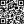
\includegraphics[width=0.8\textwidth]{qr_github_tofa.pdf}\par}
\vspace{0.2em}
{\small{\ml{$0$}{О книге и авторе}{About the book and the author}}\par}
}
\end{minipage}
\hspace{2em}
\begin{minipage}[t]{0.25\textwidth}
{\centering
{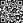
\includegraphics[width=0.8\textwidth]{qr_license_by40.pdf}\par}
\vspace{0.2em}
{\small{\ml{$0$}{Текст лицензии}{License full text}}\par}
}
\end{minipage}
\hfill}
% ----- QR CODES -----

% }
% % ----- INFO PAGE -----
%
% % ----- EMPTY PAGE -----
% \newpage\thispagestyle{plain}~
% % ----- EMPTY PAGE -----
%
% % ----- BACK COVER -----
% 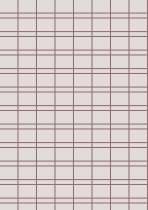
\includepdf[pages={1}]{cover_back.pdf}
% % ----- BACK COVER -----

\end{document}
